\documentclass[12pt,xcolor=x11names,compress, notes=show]{beamer}% pour l'impression, tout n'apparait qu'une fois \documentclass[handout,12pt]{beamer}
\usepackage[utf8x]{inputenc}
\usepackage{ucs}
\usepackage[french]{babel}
\usepackage{todonotes}
\usepackage{tikz}
\usepackage{color}
\usepackage{subfigure}


%\usepackage{palatino}

%pour le theme
%\usetheme{CambridgeUS}

%\usetheme{Goettingen}
\useinnertheme{default}
\useoutertheme[subsection=false]{miniframes}
\setbeamertemplate{blocks}[rounded][shadow=true]
\setbeamercolor{block title}{fg=DeepSkyBlue4,bg=DeepSkyBlue4!10}
\setbeamercolor{block title alerted}{bg=DeepSkyBlue4!0} 
\setbeamercolor{block title example}{bg=DeepSkyBlue4!20}
\setbeamercolor*{lower separation line head}{bg=DeepSkyBlue4} 

\setbeamerfont{title like}{shape=\scshape}
\setbeamercolor{frametitle}{fg=DeepSkyBlue4}
\setbeamercolor{title}{fg=DeepSkyBlue4}
\setbeamercolor{itemize item}{fg=black}
\setbeamercolor{itemize subitem}{fg=black}
\setbeamercolor{toc}{fg=DeepSkyBlue4}

%couleur table des matières
\usepackage{hyperref}
\hypersetup{colorlinks=true, linkcolor=DeepSkyBlue4}

%Mettre la section courante en titre de diapo (pour champ de titre non-vide)
%\addtobeamertemplate{frametitle}{\frametitle{\insertsubsectionhead}}{}

\addtobeamertemplate{footline}{\hspace{11cm} \insertframenumber/\inserttotalframenumber}

\author{Alice \textsc{Dinsenmeyer} \& Thomas \textsc{Lechat} \\ encadrés par Olivier \textsc{Richoux}}

\title{ Réseaux acoustiques et modes localisés}
\subtitle{M1 Acoustique}
\date{\today}



\begin{document}

\begin{frame}
	\titlepage 
\end{frame}



\section*{Introduction}
\begin{frame}{\insertsectionhead}

\begin{itemize}
\item Objectif : observer expérimentalement un mode localisé
\item Contexte: méta-matériaux, applications à l'acoustique non-linéaire
\end{itemize}
	\centering
	\begin{figure}
		\centering
		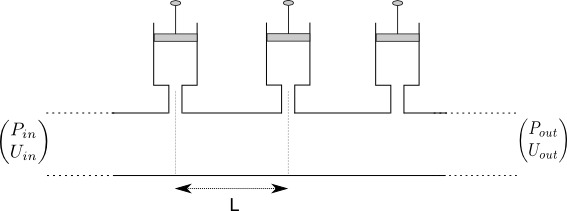
\includegraphics[height=2.5cm]{schema_reseau_infini.png}\vspace{1.3cm}\hspace{0.5cm}
		\centering
		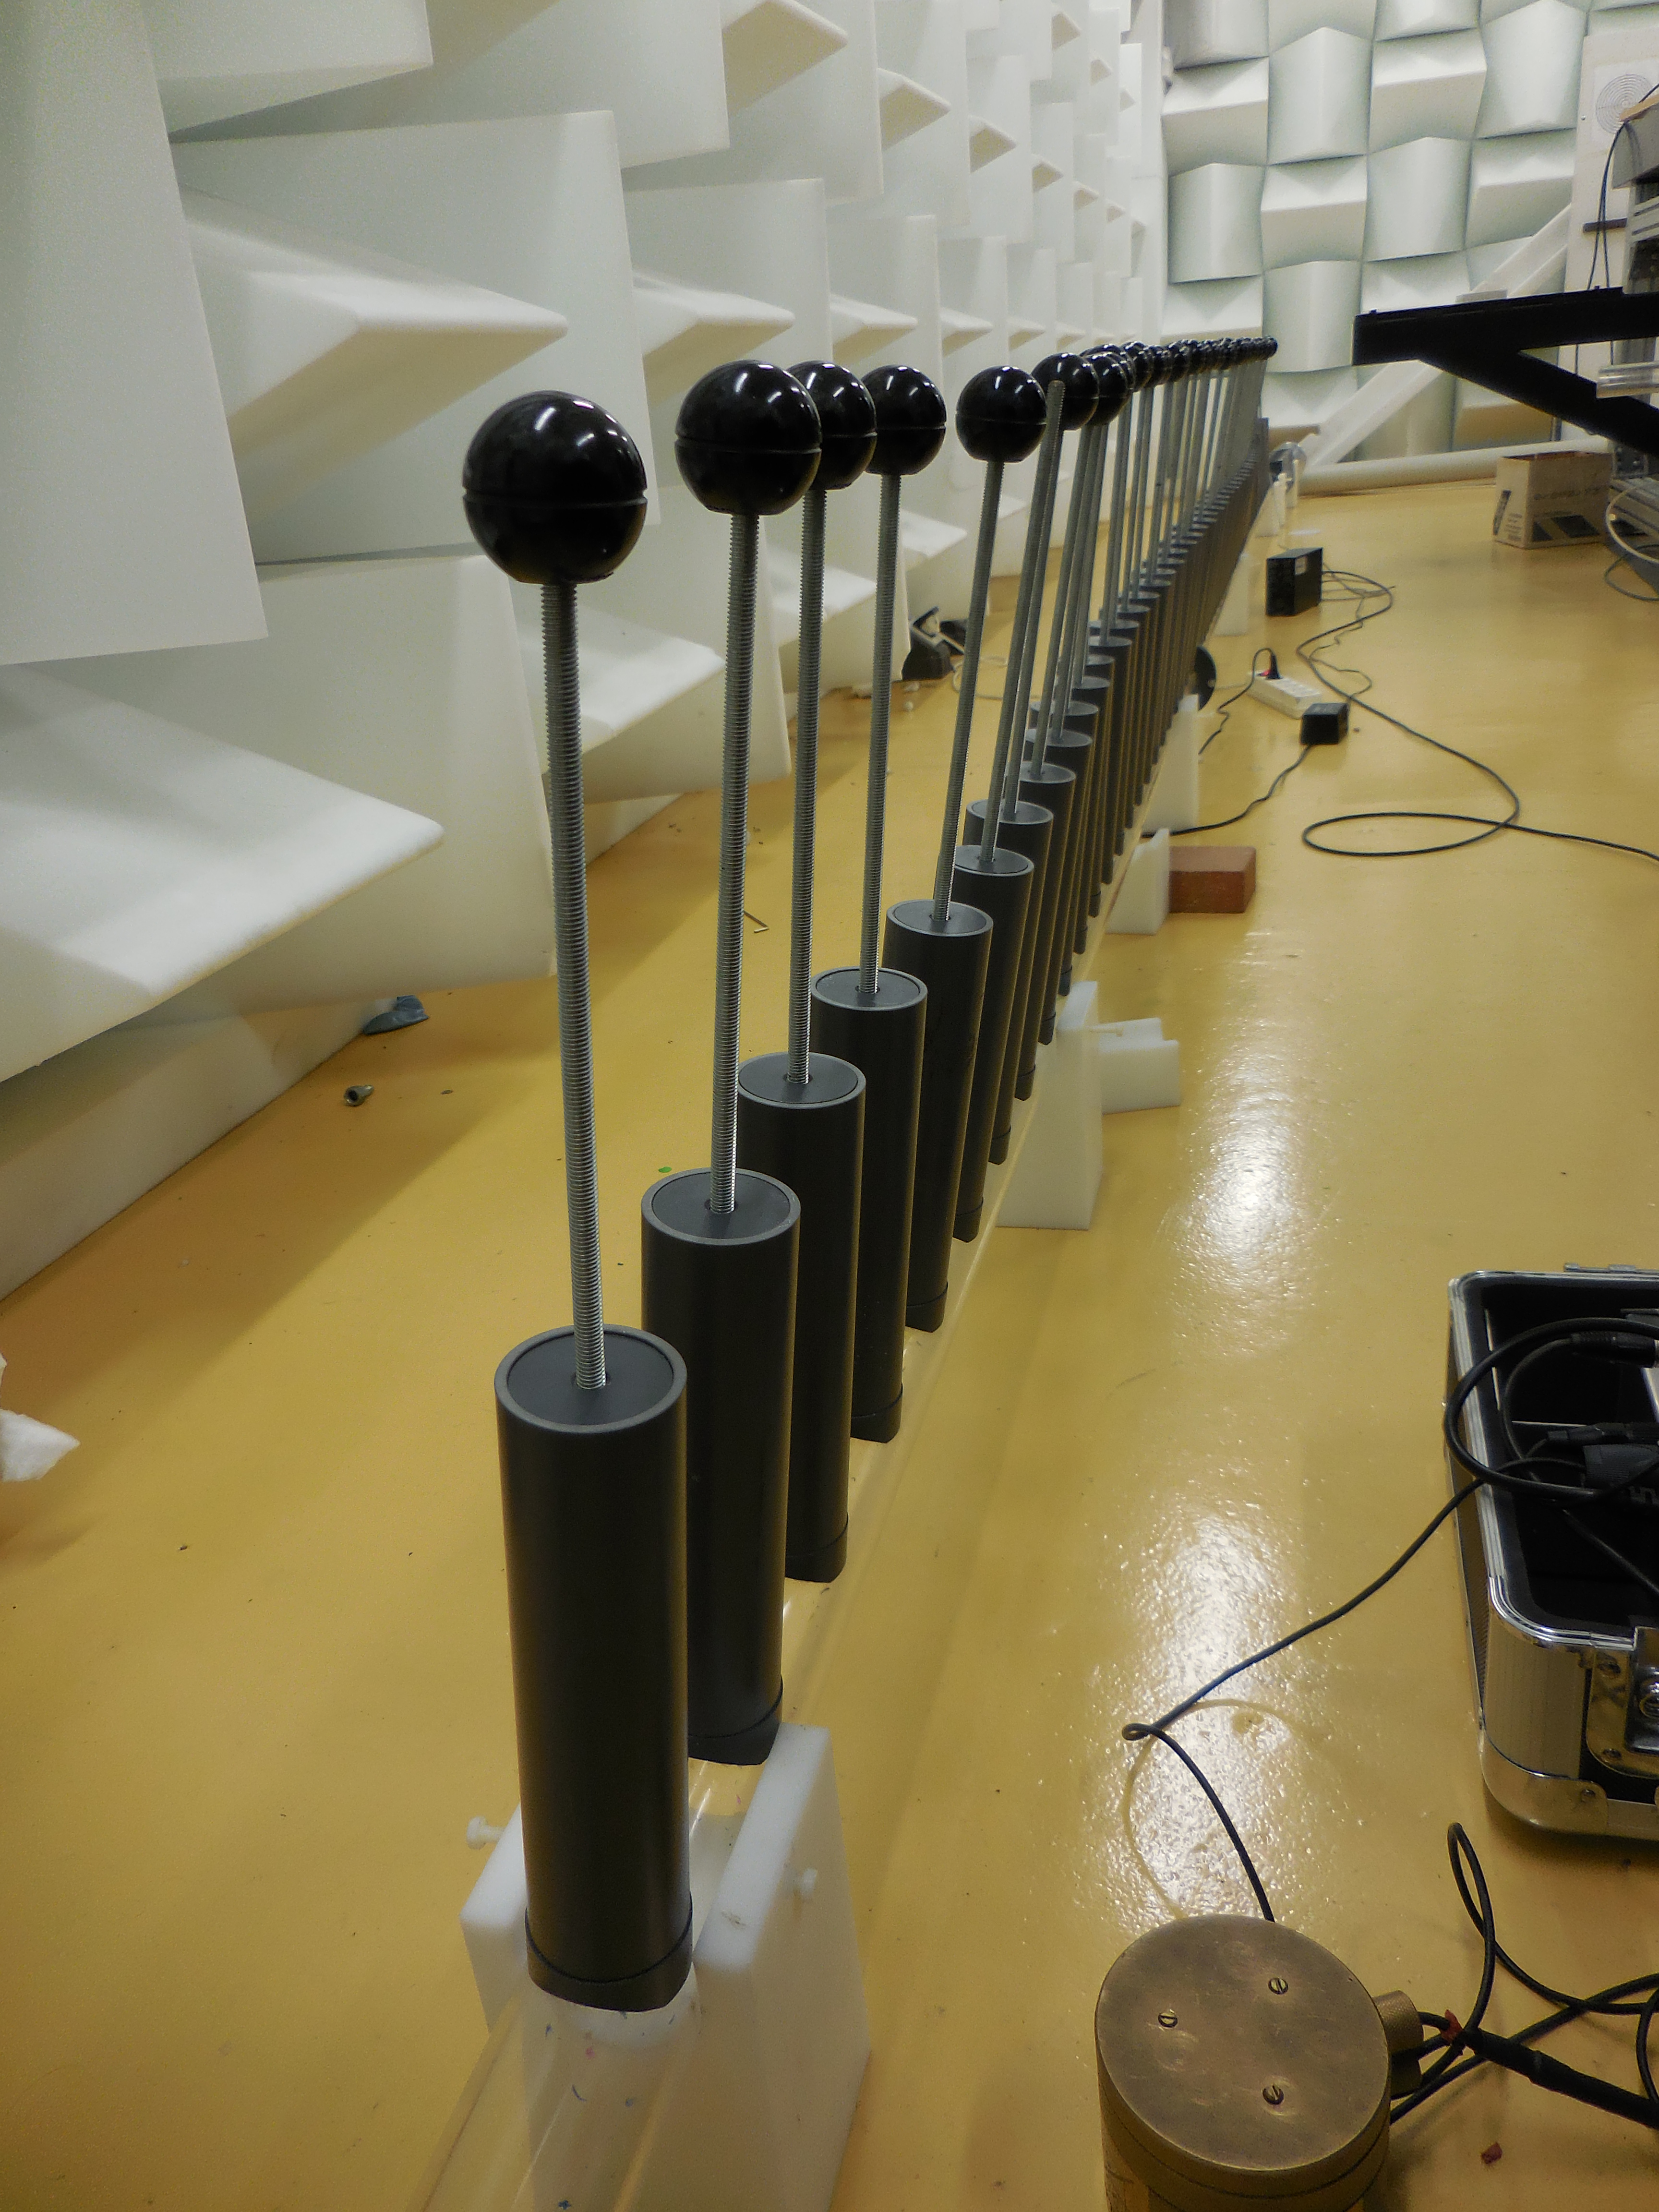
\includegraphics[height=4cm]{photo.jpg}
	\end{figure}
	
\end{frame}

\begin{frame}{Plan}
\tableofcontents[hideallsubsections]
\end{frame}


\section{Réseau infini}

\subsection{Formalisme matriciel}
\begin{frame}{\insertsectionhead : \insertsubsectionhead }
Matrices de transfert : 
\begin{itemize}
	\item pour un guide 
	\begin{eqnarray*}
	\begin{pmatrix} p_1 \\ v_1 \end{pmatrix} = \begin{pmatrix} \cos(kL) & \frac{j\omega\rho}{k} \sin(k L) \\  \frac{k}{j\omega\rho}\sin(k L) & \cos(k L) 		\end{pmatrix} 	\begin{pmatrix} p_2 \\ v_2 \end{pmatrix}
	\end{eqnarray*}
	
	\item pour un résonateur
\end{itemize}

\begin{footnotesize}
		\begin{eqnarray*}
\begin{pmatrix} P_e \\U_e \end{pmatrix}&=&\underbrace{
				\begin{pmatrix} \cos(k L_n) & j Z_{n} \sin(k L_n) \\ \frac{1}{Z_{n}} \sin(k L_n) & \cos(k L_n) \end{pmatrix}}_{\text{\normalsize Col}}
				\underbrace{\begin{pmatrix} \cos(k L_c) & j Z_{c} \sin(k L_c) \\ \frac{1}{Z_{c}} \sin(kL_c) & \cos(k L_c) \end{pmatrix}}_{\text{\normalsize Cavité}}
				 \begin{pmatrix} P_s \\ 0  \end{pmatrix}
		\end{eqnarray*}
\end{footnotesize}

\end{frame}




%\begin{frame}{~}
%Ajout des pertes viscothermiques: changement sur $k$ et $Z_c$
%\begin{eqnarray*}
% k =  \frac{\omega}{c_0} \left( 1 + \frac{\beta}{s}(1+(\gamma-1)/ \chi \right) \\
% Z_c =  \frac{\rho c_0}{S} \left( 1 + \frac{\beta}{s}(1-(\gamma-1)/ \chi \right) 
%\end{eqnarray*}
%
%Dans ces expressions, on a:
%\begin{itemize}
% \item  $s=R/ \delta$ avec $\delta = \sqrt{\frac{2 \mu}{\rho \omega}}$
% \item  $\chi = \sqrt{P_r}$ ou $P_r$ est le nombre de Prandtl
% \item $\beta = (1-j)/\sqrt{2}$ 
% \item $\mu$ la viscosité de l'air
%\end{itemize}
%\end{frame}


\subsection{Bande interdites}
\begin{frame}{\insertsectionhead : \insertsubsectionhead}
\vspace{0.3cm}


	\begin{columns}[T]
		
		\column{0.3 \textwidth}
		\centering
 		Résonance du résonateur de Helmholtz\vspace{-0.2cm}
 		\flushright
		\begin{tikzpicture}
			\draw[line width=1pt,black!70,->] (0,0) --  (0.4,-0.7);
 		\end{tikzpicture}
		
		\column{0.3 \textwidth}
		\centering
		Résonance de la cavité du résonateur \vspace{-0.2cm}
		\flushleft
		\begin{tikzpicture}
			\draw[line width=1pt,white] (0,0) -- (2,0);
			\draw[line width=1pt,black!70,->] (2,0) --  (2.5,-0.7);
 		\end{tikzpicture}

 		
 		\column{0.3 \textwidth}
 		\centering
 		Périodicité \\(bande de Bragg)\\~\vspace{-0.2cm}
 		\flushleft
 		\begin{tikzpicture}
 			\draw[line width=1pt,white] (0,0) -- (1,0);
			\draw[line width=1pt,black!70,->] (1.2,0) --  (0.9,-0.7);
 		\end{tikzpicture}
	
	\end{columns} 
\vspace{-0.3cm}
	\begin{figure}
		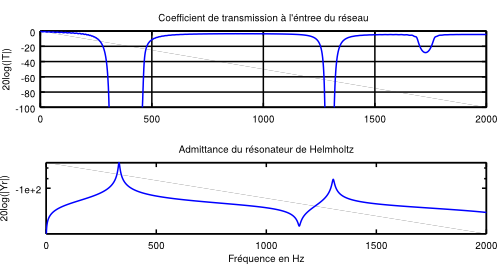
\includegraphics[scale=0.45]{transmission.png}
	\end{figure}
	

\end{frame}


\section{Ajout d'une singularité}
\begin{frame}{\insertsectionhead}

	Ajout d'une \textbf{singularité} sur un des résonateurs\\
	  \hspace{1cm} $\hookrightarrow$ création d'un mode localisé \\

	\vspace{1cm}
	\begin{block}{Problématique}
		\begin{itemize}
			\item Où placer cette singularité ?
			\item Comment choisir sa fréquence de résonance ?
			\item Comment l'observer expérimentalement ?
		\end{itemize}
	\end{block}
 
\end{frame}


\subsection{à quelle fréquence ?}
\begin{frame}{\insertsectionhead : \insertsubsectionhead}
\begin{columns}[T]
	\column{0.5 \textwidth}
	 Hors d'une bande interdite : réflexion totale 
	\begin{figure}
		\centering
		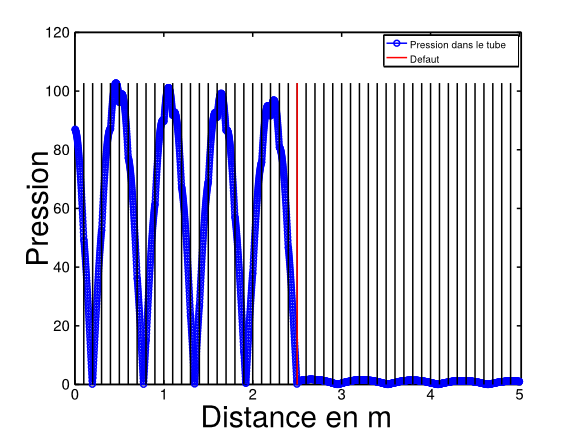
\includegraphics[width=\textwidth]{horsbande_50RH_500Hz_71mm.png}
	\end{figure}
	
	\column{0.5 \textwidth}
	 Dans une bande interdite : localisation de l'onde
	\begin{figure}
		\centering
		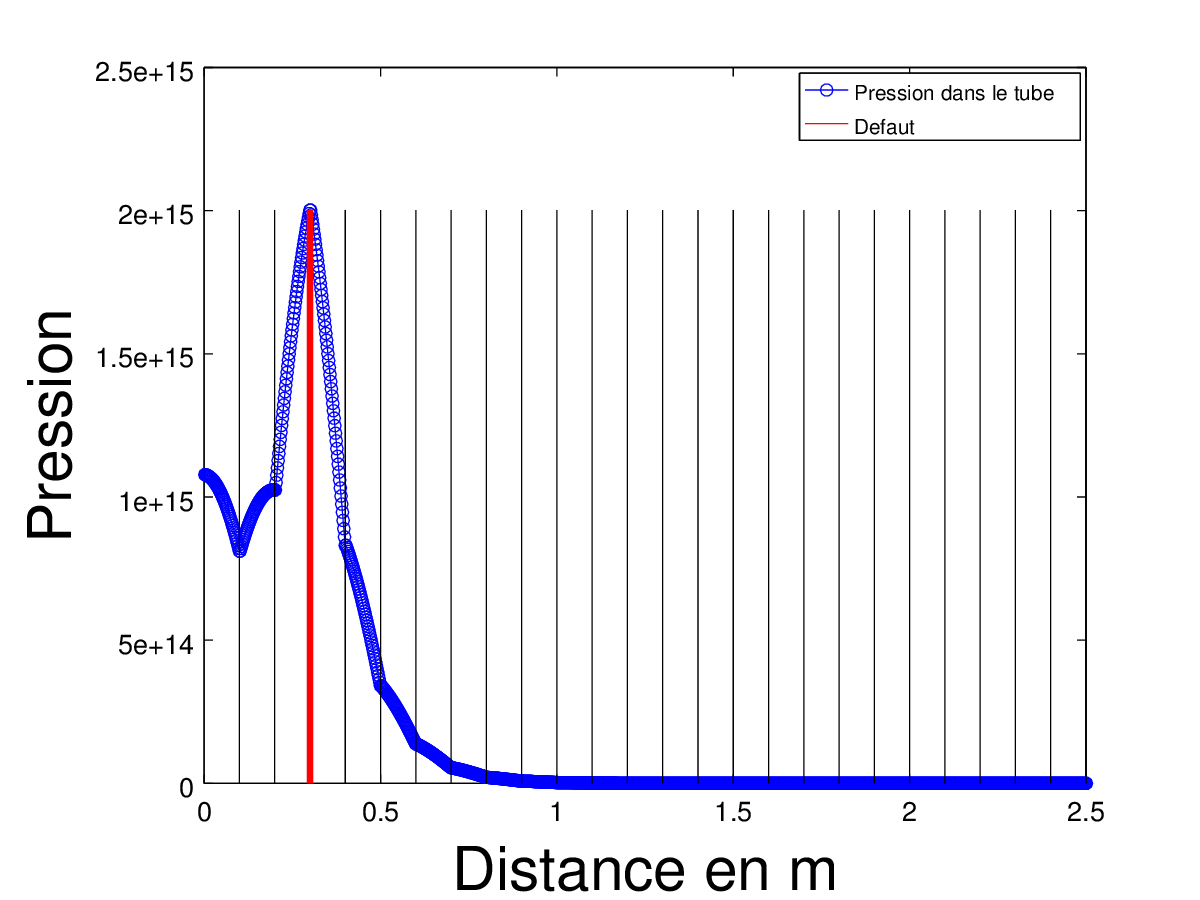
\includegraphics[width=\textwidth]{visu_pression_favo2.png}
	\end{figure}
\end{columns}
\end{frame}

\subsection{à quelle position ?}
\begin{frame}{\insertsectionhead : \insertsubsectionhead}


Transmission en fonction de la position :
\begin{figure}
	\centering
	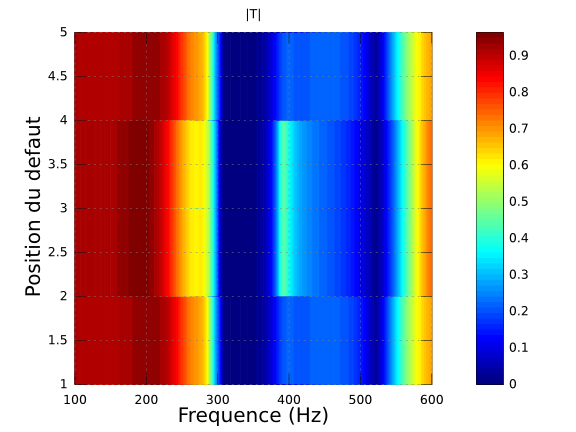
\includegraphics[scale=0.5]{pos_singu.png}
\end{figure}
\end{frame}



\subsection{réflexion et transmission}
\begin{frame}{\insertsectionhead : \insertsubsectionhead}
Sans défaut :
\vspace{-0.3cm}
\begin{figure}
\centering
\subfigure[Réflexion]{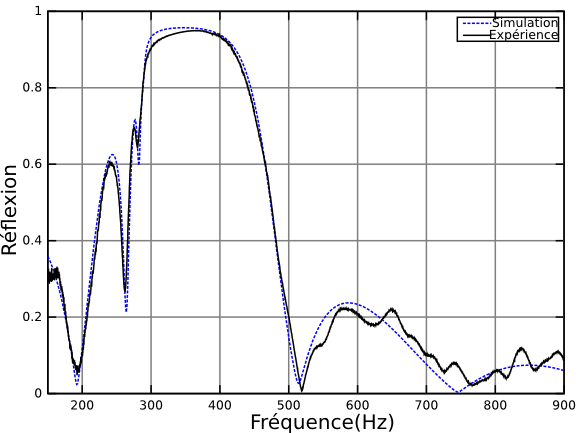
\includegraphics[width=0.35\textwidth]{R_5HR165_nodefect}}
\subfigure[Transmission]{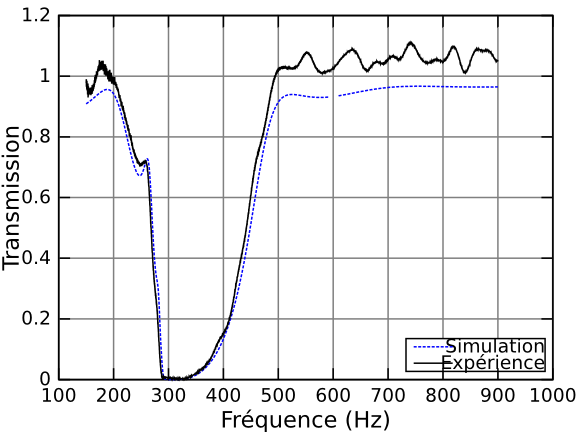
\includegraphics[width=0.35\textwidth]{T_5HR165_nodefect.png}}
\end{figure}

Avec défaut (bord de bande interdite) : 
\vspace{-0.3cm}
\begin{figure}
\centering
\subfigure{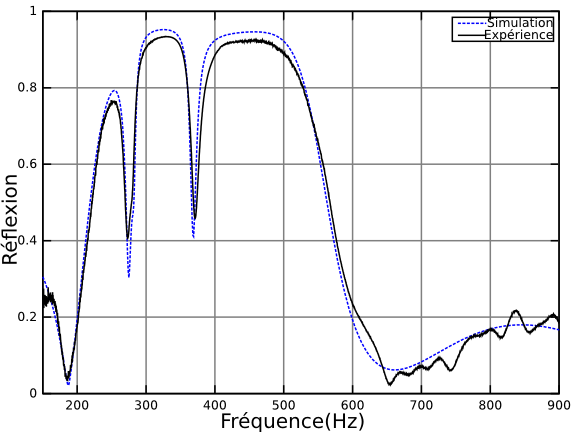
\includegraphics[width=0.35\textwidth]{R_5HR165_8cm_pos3.png}}
\subfigure{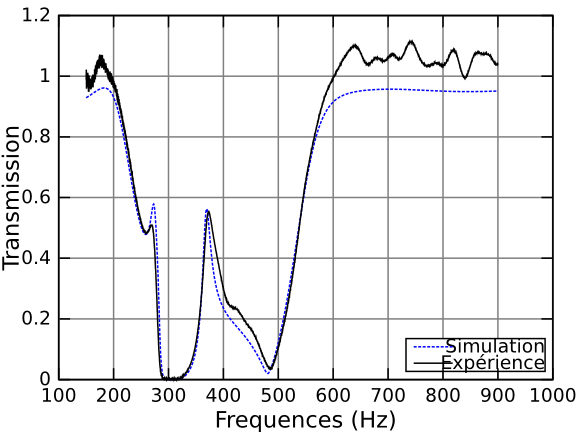
\includegraphics[width=0.35\textwidth]{T_5HR165_8cm_pos3.png}}
\end{figure}


\end{frame}

\section{Visualisation expérimentale du mode localisé}

\begin{frame}{\insertsectionhead}

\begin{figure}
\centering
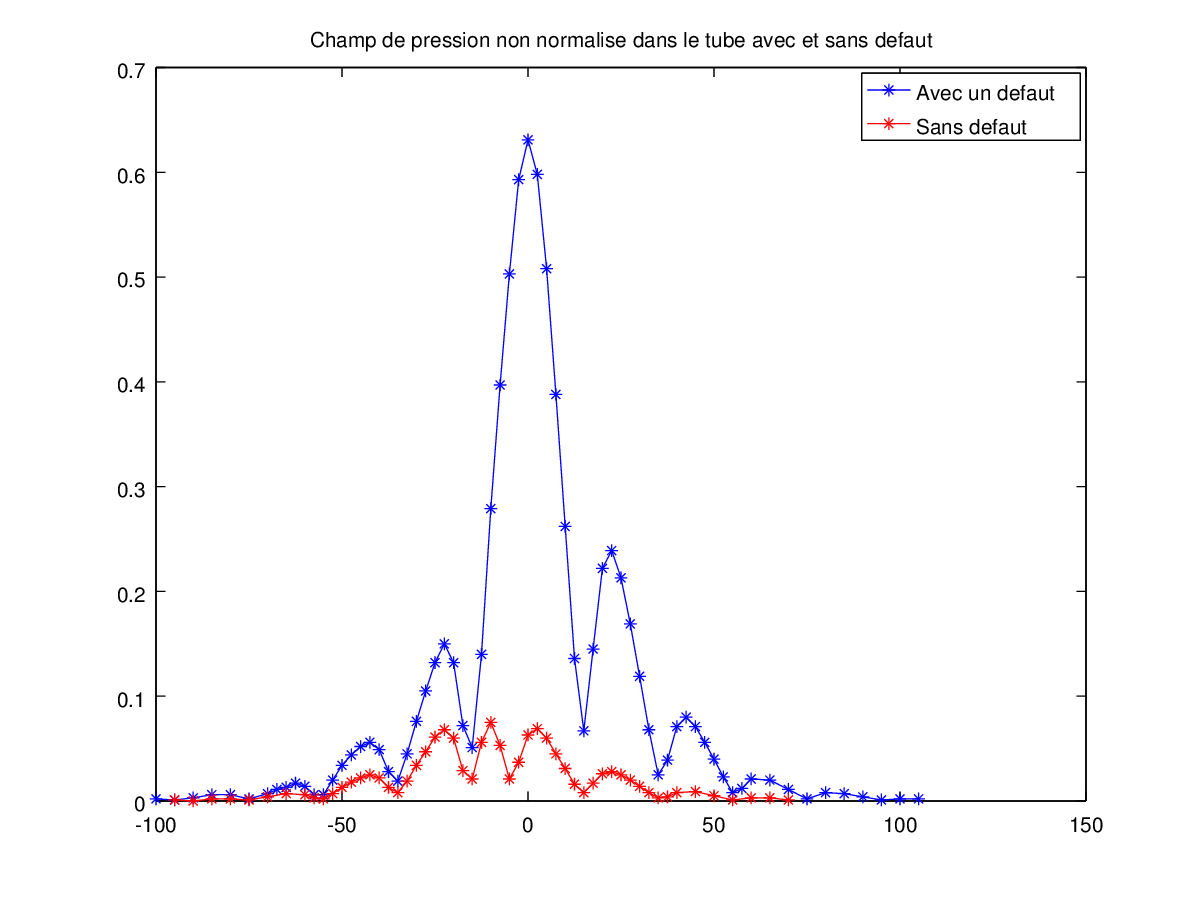
\includegraphics[scale=0.4]{non_norm_lin.png}
\end{figure}

\begin{center}
	Pression mesurée dans le réseau.
\end{center}

\end{frame}


\subsection{Changement de géométrie du réseau}
\begin{frame}{\insertsectionhead}
\insertsubsectionhead\\~\\

Ajout d'un 2\textsuperscript{ème} défaut $\rightarrow$ symétrie
\vspace{-0.5cm}
\begin{columns}[T]
	\column{0.5 \textwidth}
	\begin{figure}
		\centering
		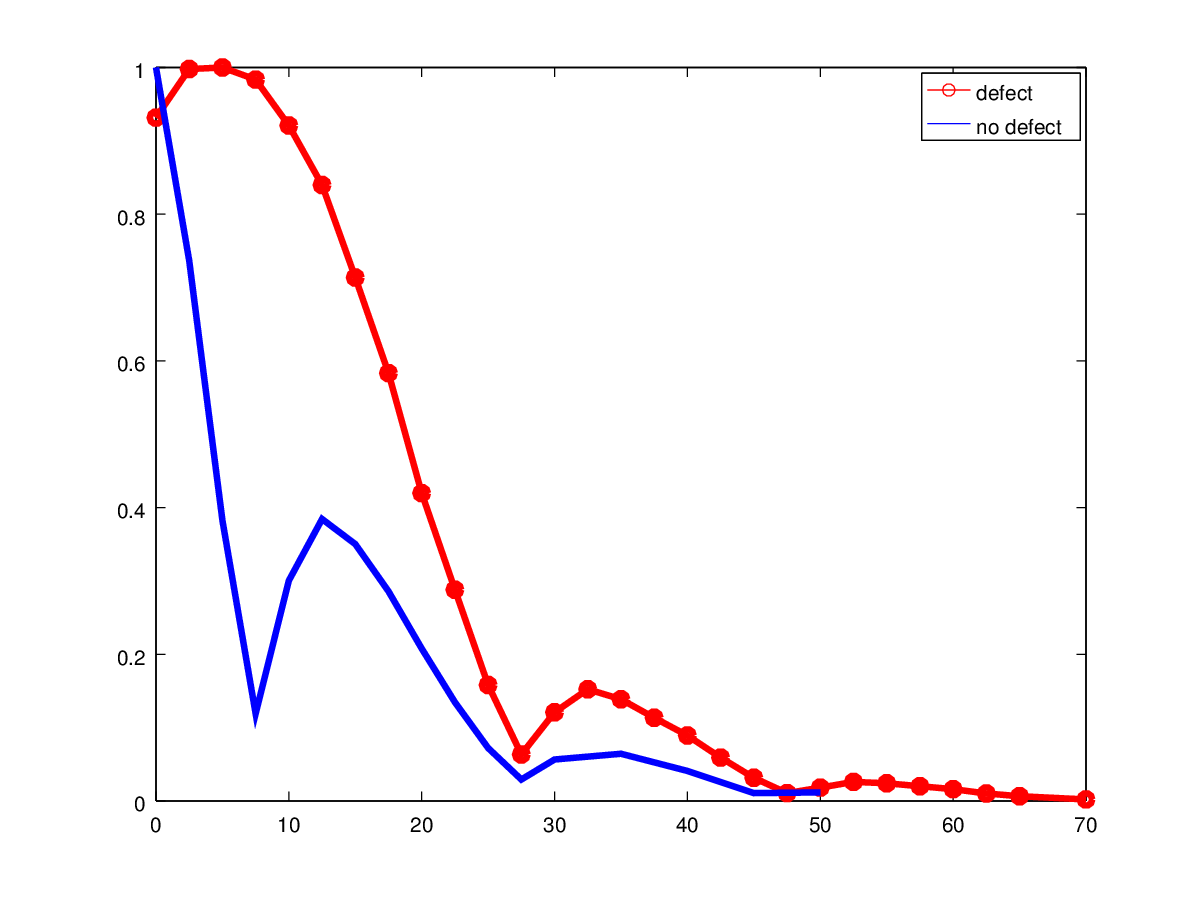
\includegraphics[height=0.5\textheight]{comparaison_decroissance_lin.png}
	\end{figure}
	\centering
	\footnotesize{Échelle linéaire.}
	
	\column{0.5 \textwidth}
	\begin{figure}
		\centering
		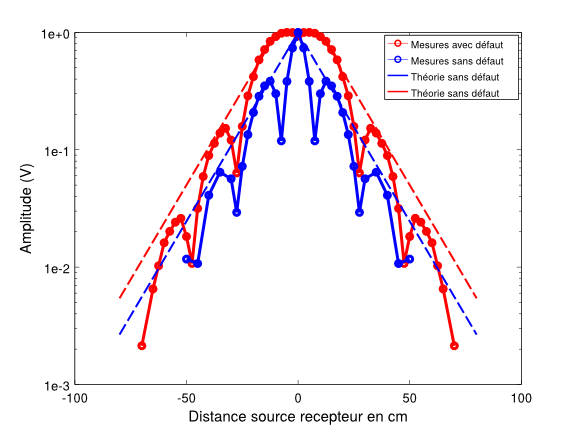
\includegraphics[height=0.5\textheight]{comparaison_decroissance_log_theo.png}
	\end{figure}
	\centering
	\footnotesize{Échelle logarithmique, amplitude normalisée.}
\end{columns}
\end{frame}


\section*{Conclusions}
\begin{frame}{\insertsectionhead}

%ouvertures
\begin{itemize}
	\item Forte amplitude locale $\rightarrow$ effets non-linéaires possibles\\~\\
	\item Applications en acoustique non-linéaire : 
		\begin{itemize}
			\item[•] filtrage dynamique,
			\item[•] système asymétrique, 
			\item[•] conception de matériaux variés.
		\end{itemize}
\end{itemize}

	
\end{frame}

\begin{frame}{Bibliographie}
\indent J P Dalmont. Guide des Guides d'ondes acoustiques (version 1.4). 2010 \\ ~\\
\indent O Richoux. Étude de la propagation des ondes mécaniques dans un réseau unidimensionnel comportant du désordre et/ou des non-linéarités localisées. Th. doct. : Acoustique. Le Mans : université du Maine, 1999 \\~\\
\indent G Theocharis, O Richoux, V Romero García, A Merkel, and V Tournat. Limits of slow sound propagation and transparency in lossy, locally resonant periodic structures. New Journal of Physics, 2014.


\end{frame}


\end{document}